\section{Introduction}

% JT: Trying to write short, as we have only 8 pages.
%\JT{EVERYONE: I am a bit concerned about two reductionist arguments that will be thrown at us: 1. why don't we just try and make the initial segmentation better? 2. at the limit, someone still has to scan the whole volume because your edge error classifier is often wrong. Any ideas?}

%Paragraph one: Provide context to the work.
%What is the task? What is the state of the task?
In connectomics, neuroanatomists \change{annotate neurons and their connectivity within 3D volumes} to gain insight into the functional structure of the brain. Rapid progress in automatic sample preparation and electron microscopy (EM) acquisition techniques has made it possible to image large volumes of brain tissue at $\approx6\, nm$ per pixel to identify cells, synapses, and vesicles. For $25\, nm$ thick sections, a $1\, mm^3$ volume of brain contains $10^{15}$ voxels, or 1 petabyte of data. \change{With so much data,} manual annotation is infeasible, and automatic annotation methods are needed \cite{jain2010,Liu2014,GALA2014,kaynig2015large}.

Automatic annotation by segmentation and classification of brain tissue is challenging \cite{isbi_challenge}. The state of the art uses supervised learning with convolutional neural networks \cite{Ciresan:2012f}, or potentially even unsupervised learning \cite{BogovicHJ13}. \change{Typically, cell membranes are detected in 2D images, and the resulting region segmentation is grouped into geometrically-consistent cells across registered sections. Cells may also be segmented across registered sections in 3D directly.} Using dynamic programming techniques \cite{Masci:2013a} and a GPU cluster, these classifiers can segment $\approx1$ terabyte of data per hour \cite{kasthuri2015saturated}, which is sufficient to keep up with the 2D data capture process on state-of-the-art electron microscopes (though 3D registration is still an expensive offline operation).
% \cite{Ciresan:2012f,RonnebergerFB15,lee2015recursive}

%State of the art methods use convolutional neural networks to learn cell membranes in 2D images from hand-labeled training data. Then, labeled membranes are grouped into geometrically-consistent cell regions across sections to form 3D image stacks. Using dynamic programming techniques \VKF{cite cdd whole image training paper}, and small GPU clusters \VKF{how many?}, these classifiers can segment about 1 terabyte of data per hour \cite{kasthuri2015saturated,lee2015recursive}, which is the rate necessary to keep up with the data capture process on state-of-the-art electron microscopes. %\VKF{citation for 61 beam microscope?}. \JT{I would skip. There is a Nature press piece (see comment in source), but is there a peer-reviewed academic article? Also, I cited the recent Cell paper for the segmentation rates above; I hope that is ok.} % \url{http://www.nature.com/nature/journal/v503/n7474/full/503147a.html?WT.ec_id=NATURE-20131107}

%Paragraph two: What is the problem in this context? What is the situation that you are trying to correct or overcome?
All automatic methods make errors, and we are left with large data which needs \emph{proofreading} by humans. This crucial task serves two purposes: 1) to correct errors in the segmentation, and 2) to provide a large body of labeled data to train better automatic segmentation methods. Recent proofreading tools provide intuitive user interfaces to browse segmentation data in 2D and 3D and to identify and manually correct errors \cite{markus_proofreading,raveler,mojo2,haehn_dojo_2014,karimov_guided_volume_editing,uzunbas}. Many kinds of errors exist, such as inaccurate boundaries, but the most common are \emph{split errors}, where a single cell is labeled as two, and \emph{merge errors}, where two cells are labeled as one (Fig.~\ref{fig:merge_error}). With user interaction, split errors can be joined, and the missing boundary in a merge error can be defined with manually-seeded watersheds \cite{haehn_dojo_2014}. However, even with semi-automatic correction tools, the visual inspection to find errors in the first place takes the majority of the time.

\begin{figure}[t]
\centering
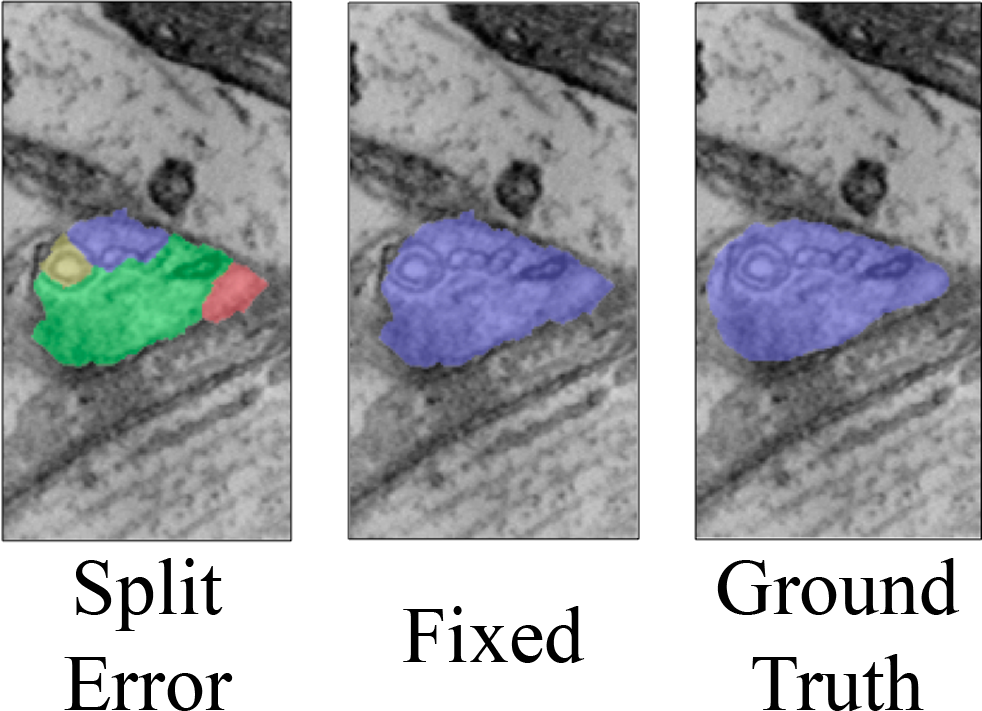
\includegraphics[width=.35\textwidth]{gfx/spliterror_2.png}
\qquad
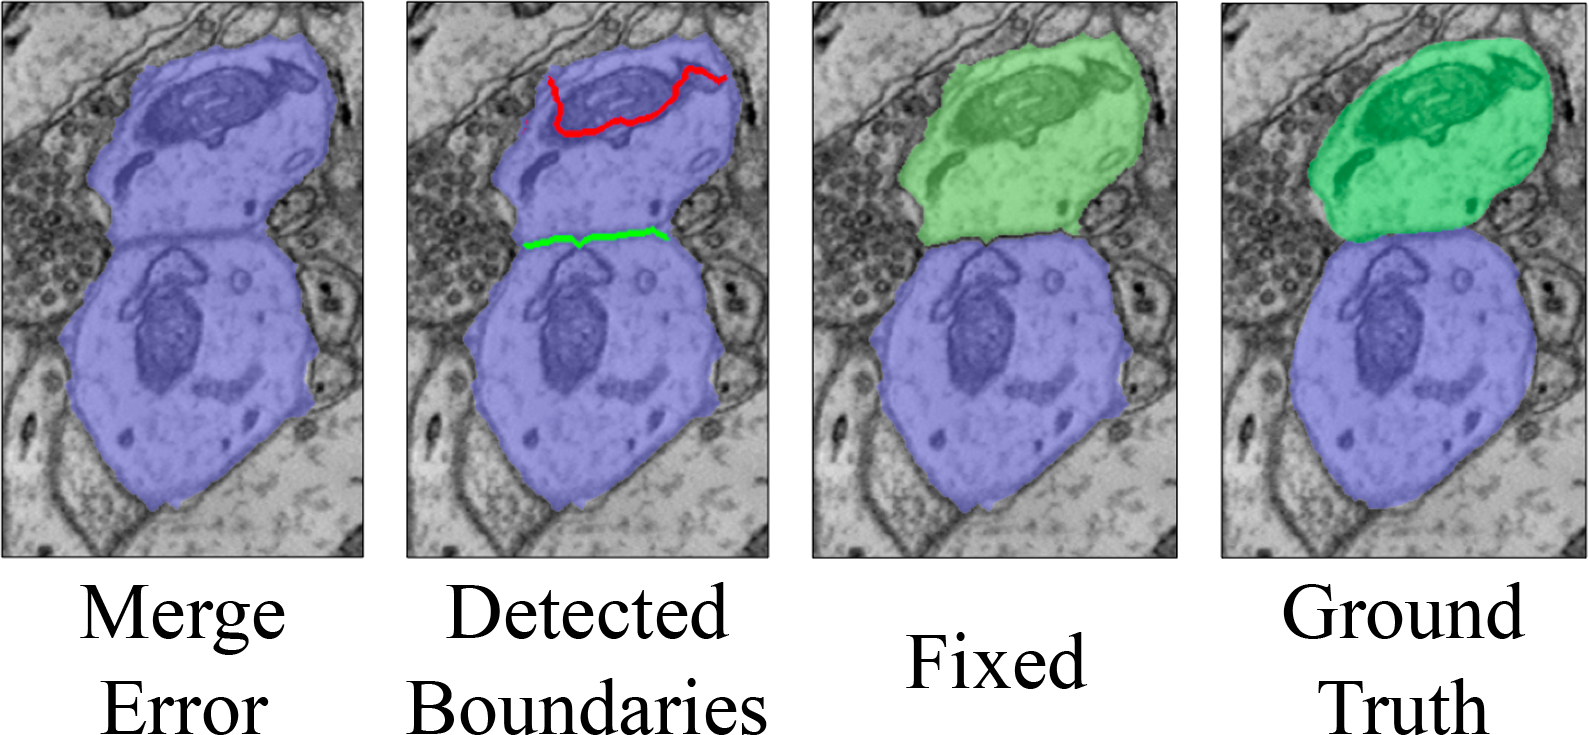
\includegraphics[width=.55\textwidth]{gfx/mergeerror.png}
\caption{Split and merge error examples, their corrections, and their ground truths.}
\label{fig:merge_error}
\end{figure}

%Paragraph three: What is the proposed solution at a high level? What is the result of the method, and how does it impact the problem?
Our goal is to add automatic detection of split and merge errors to proofreading tools. Instead of the user visually inspecting the whole data volume carefully to spot errors, we design automatic classifiers that detect split and merge errors in 2D segmentations. Then, a proofreading tool can recommend regions with a high probability of an error to the user, and suggest corrections to accept or reject. We call this process \textit{Guided Proofreading}.

% JT: Cut, as it was confusing. Sufficient to be without, as the end of the paragraph makes it clear.
%The initial automatic segmentation is constrained by the data rate of the microscope.  , which relaxes the constraint on speed

\change{Given a membrane segmentation from a fast automatic method, our classifiers operate on the boundaries of whole cell regions. Compared to techniques that must analyze every input pixel, we reduce the data analysis to the boundaries only. This allows us to employ wider convolutional neural networks that take regional context and multiple input channels into account.} One reason to classify errors on 2D images lies with the cost of 3D registration. This is often slow as it requires non-linear image alignment \cite{akselrod09,Saalfeld2010Asrigidaspossible}. However, typically segmentation results are local decisions at the cell level. In this case, 3D reconstruction is unnecessary and, instead of waiting for the 3D output, proofreading can start immediately to maximize error correction before cell grouping occurs across sections.

%Paragraph five: Optimistically, what is the consequence of the method - what can I do now that I could not do before?
We quantitatively validate our approach with variation of information (VI) versus ground truth expert segmentations. While unintuitive, VI is a common metric to evaluate region segmentation performance \cite{NunezIglesias2013Machine}. We compare our approach \change{to} an existing proofreading tool that provides only semi-automatic merge error correction~\cite{haehn_dojo_2014}. With a simulated user, our automatic error suggestions and corrections decrease VI from 0.4764 to 0.3996, which is in contrast to pure manual or pure automatic methods that can both \emph{increase} VI. \change{On a second larger dataset}, our method decreases VI from 0.4847 to 0.3946. As a consequence, we are able to provide tools to proofread segmentations more efficiently, and so better tackle large volumes of connectomics imagery.

%\subsection{Contributions}
%
%Given this, we contribute to the literature:
%\begin{enumerate}
%\item One contribution
%\item Two contribution
%\item (Maybe) three contribution
%\end{enumerate}
%
%\begin{figure}
%\missingfigure{Example of a fixed split error. Example of a fixed merge error.}
%\caption{Example of a fixed split error. Example of a fixed merge error.}
%\end{figure}